\documentclass[conference]{IEEEtran}
\IEEEoverridecommandlockouts
% The preceding line is only needed to identify funding in the first footnote. If that is unneeded, please comment it out.
\usepackage{cite}
\usepackage{titlesec}
\usepackage{amsmath,amssymb,amsfonts}
\usepackage{algorithmic}
\usepackage{graphicx}
\usepackage{textcomp}
\usepackage{xcolor}
\def\BibTeX{{\rm B\kern-.05em{\sc i\kern-.025em b}\kern-.08em
    T\kern-.1667em\lower.7ex\hbox{E}\kern-.125emX}}
\begin{document}

\title { \HUGE {Kocaeli Üniversitesi}\\
\LARGE {Bilgisayar Mühendisliği Bölümü}\\
\huge \textbf{Programlama Laboratuvarı 1}\\
\LARGE{Proje 3}\\
\LARGE{Havalimanı Uçuş Yönetim Sistemi}
}

\author
{
\IEEEauthorblockN{\large Robera Tadesse GOBOSHO}
\IEEEauthorblockA{\large ID:190201141\\
\textit{\large robtad318@gmail.com}}


\and
\IEEEauthorblockN{\large Muhammad Abdan SYAKURA}
\IEEEauthorblockA{\large ID:200201147\\
\textit{\large prof.syakur@gmail.com }}
}


\maketitle
\section*{\textbf{\LARGE Özet}}
\Large{ Bu rapor Programlama Laboratuvarı 1 dersi 3. Projesinin çözümünü açıklamak üzere hazırlanmıştır. Bu proje C diliyle yapılmıştır. Öncelikli kuyruk (priority queue) uygulanarak İstanbul Havalimanı için bir havalimanı uçuş yönetim sistemi geliştirilmiştir.
Öncelikle havalimanına inmek için talep eden uçaklar “input.txt” dosyasından okunmaktadır. Dosya içerisinde oncelik\_id, ucak\_id ve talep\_edilen\_inis\_saati 3 tane giriş bulunmaktadır ve tek tek satırları okunmaktadır. Her satır okunurken talep edilen iniş saatine bakılır ve kontrol edilir. Eğer daha önce aynı saatte başka uçak talep etmişse, iki uçağın öncelik id’lerine karşılaştırılır. Hangisi daha yüksek öncelik id’ye sahip ise o uçak talep edilen saatte iniş yapacaktır. Diğer uçak ise 1 saat ertelenir. Ve ertelendikten sonraki saati de kontrol edilecektir.  O saatte aynı uçak varsa aynı işlem görülecektir. Eğer iki uçağın talep edilen saati ve öncelik id’si aynı ise bu durumda uçak id’lerini kontrol edilir. Eğer bir uçak 3 kereden fazla ertelenirse o uçak iniş için Sabiha Gökçen Havalimanı’na yönlendirilir. Ve bir günde sadece 24 tane uçak iniş için izin isteyebilmektedir. Bu işlemler de input dosyasının son satırına kadar devam edecektir. 
Kalkış için de iniş saatlerinden 1 sonraki saat yapılır. İnişleri düzeldiği için kalkışta saat çakışması söz konusu değildir. Bu işlemler de “output.txt” dosyasına aktarılır. Dosya içerisinde 6 tane bilgi içermektedir: oncelik\_id, ucak\_id, talep\_edilen\_inis\_saati, inis\_saati, gecikme\_suresi, kalkis\_saati.
}

\section*{\textbf{\LARGE Gİrİş}}
\Large{
1 iniş 1 kalkış olmak üzere 2 pisti bulunan İstanbul Havalimanı’nda gün içerisinde (1-24 saat dilimi boyunca) yapılan uçuşların yönetimi için bir sistem geliştirildi. Havalimanında aynı anda sadece 1 uçak kalkış yapabiliyorken sadece 1 uçak iniş yapabilmektedir. Uçakların her biri önceliklere sahiptir ve 1 günde maksimum 24 uçak iniş için izin isteyebilmektedir. Havalimanındaki uçakların öncelik sırası, iniş saati, gecikme süresi ve kalkış saati bilgileri kullanılarak; iniş pistini ve kalkış pistini kullanım sırasının belirlenmektedir.

Bu projede öncelikli kuyruk kullandık. Öncelikle kuyruk, ilk giren eleman ilk çıkar (First In First Out – FIFO) mantığında çalışan bir veri yapısıdır. Örneğin, kuyruk veri yapısı bankada işlem yaptırmak için sıraya girmiş insanlara benzetilebilir. Sıraya ilk giren kişi ilk işlem yaptıracaktır. Kuyruk tasarımı için dizi ya da bağlı liste kullanılabilir. Dizi kullanılan sabit boyutlu, bağlı liste kullanılarak değişken boyutlu kuyruk oluşturulabilir. Kuyrukta işlemler iki uçtan yapılır. Kuyruk veri yapısında yapılabilecek işlemlerden bazıları aşağıdaki gibidir:

\begin{itemize}

\item enqueue(): Kuyruğun önüne eleman ekler.
\item dequeue(): Kuyruğun sonundan eleman çıkarır.
\item peek(): Silme işlemi uygulamadan sıradaki elemanı (front işaretçisinin gösterdiği düğüm) döndürür.

\end{itemize}

Öncelikli kuyruk ise bazı problemlerin çözümünde doğrudan kuyruk oluşturulamaz. Örneğin; bir hastanede muayene sırasına girmiş insanlar arasında durumu acil olan birisi bulunabilir ve bu kişi muayene için öncelikli hale gelebilir. Bu gibi durumlarda öncelikli kuyruk kullanılır. Öncelikli kuyrukta ilk giren ilk çıkar mantığı geçerli değildir, önemli olan önceliktir. Öncelikli kuyruk veri yapısında yapılabilecek işlemlerden bazıları aşağıdaki gibidir:

\begin{itemize}

\item add(): Kuyruğa eleman eklemek için kullanılır.
\item poll(): Kuyruktaki son elemanı döndürür ve elemanı kuyruktan siler.
\item peek(): Kuyruktaki son elemanı silmeden döndürür.
\item clear(): Kuyruktaki bütün elemanları siler.
\item remove(): Kuyruktaki belirtilen elemanı siler.

\end{itemize}

Öncelikli kuyruk, bir dizi, bağlı liste, heap veri yapısı veya ikili arama ağacı kullanılarak uygulanabilir. Bu veri yapıları arasında heap veri yapısı, öncelik kuyruğunu verimli bir şekilde uygulanmasını sağlar. Heap’te bir veri eklemek ve silmek için en kötü durumu O(Log n)’dir. Bundan dolayı bu projede heap veri yapısını kullandık.
}


\section*{\textbf{\LARGE Yöntem}}

%\subsection{\textbf{\Large Tanım}}\label{SCM}
İlk olarak readInput fonksiyonuyla input dosyasını okunur. Eğer aynı dizinde input dosyası bulunmuyorsa veya dosya açarken bir hata oluyorsa Fig. 1’deki gibi bir mesaj yazılacak. Eğer bir hata yoksa Fig. 2’deki gibi program sorunsuz açılacak. Dosyanın ilk satırında başlık olduğundan ilk satırından uçakların bilgilerine atlanır. Her satır okunduğunda sırasıyla PlaneP’ye atandıktan sonra PlaneP addToLandingList fonksiyonuna gönderilir ve kontrol edilir:

\begin{figure}[h]
    \centering
    \includegraphics[scale=0.5]{img/fig1.png}
    \caption{input dosyası açarken hata varsa}
    \label{Şekil:1}
\end{figure}

\begin{figure}[h]
    \centering
    \includegraphics[scale=0.5]{img/fig2.png}
    \caption{input dosyası açmayı başardı}
    \label{Şekil:2}
\end{figure}

\begin{itemize}

\item  \textbf{ Dizi boş ise }

Front ile rear 0 olarak tanımlanır ve gönderilen uçak PlaneL’in 0. İndisine atanır. FlagM değişmediği için 1 kalır ve ekrana “İniş izin talebiniz onaylanmıştır.” Yazar.

\item \textbf{Eleman varsa ve dolu değilse}

Rear 1 artacak. Gönderilen uçak PlaneL rear’inci indisine atanır. Bundan sonra da daha önce aynı saatte iniş talep eden uçakların olup olmadığını delayHandler fonksiyonuyla halledilir. 
Bu fonksiyon dizideki tüm elemanlarını kontrol eder. Eğer daha önce aynı saatte başka uçak talep etmişse, iki uçağın öncelik id’lerine karşılaştırılır. Hangisi daha yüksek öncelik id’ye sahip ise o uçak talep edilen saatte iniş yapacaktır. Diğer uçak ise 1 saat ertelenir. Ve ertelendikten sonraki saati de kontrol edilecektir.  O saatte aynı uçak varsa aynı işlem görülecektir. Eğer iki uçağın talep edilen saati ve öncelik id’si aynı ise bu durumda uçak id’lerini kontrol edilir. Eğer bir uçak 3 kereden fazla ertelenirse o uçak iniş için Sabiha Gökçen Havalimanı’na yönlendirilir. Ekrana bir mesaj yazar.  


\item \textbf{Dizi dolu ise}

Ekrana “Inis pisti kullanim sirasi dolmustur! Acil inis kosullari kontrol ediliyor... Lutfen bekleyin...” yazar. Gönderilen uçağı en son indise atanır. Çünkü dizi MAX değerinden 1 tane daha fazla yer tanımlanmıştır. Son olarak da delayHandler4Full fonksiyonu çağırılır kontrol edilir. Priority id’si daha yüksek ise acil iniş için izin verilecektir. 


\end{itemize}
Eğer uçak iniş için izin verilirse FlagM değişmez 1 kalır ve ekrana “İniş izin talebiniz onaylanmıştır.” Yazar. Sonra da güncel kalkış pisti kullanım sırası ekrana yazdırılacaktır.

\begin{figure}[h]
    \centering
    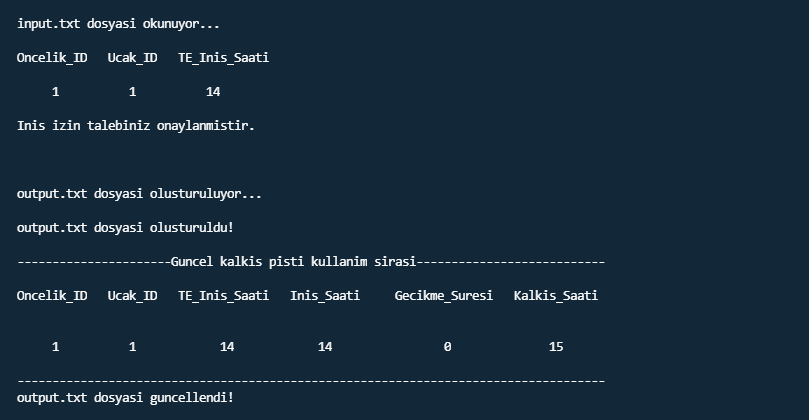
\includegraphics[scale=0.5]{img/input output for one plane.png}
    \caption{ilk uçak girdi}
    \label{Şekil:3}
\end{figure}
\begin{figure}[h]
    \centering
    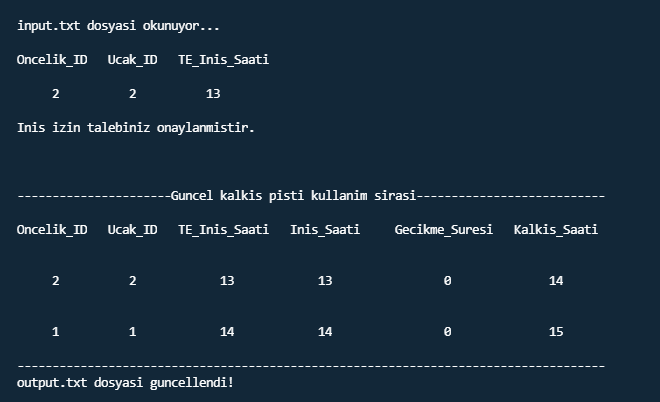
\includegraphics[scale=0.5]{img/input output for two planes.png}
    \caption{ikinci uçak girdi}
    \label{Şekil:4}
\end{figure}
\begin{figure}[h]
    \centering
    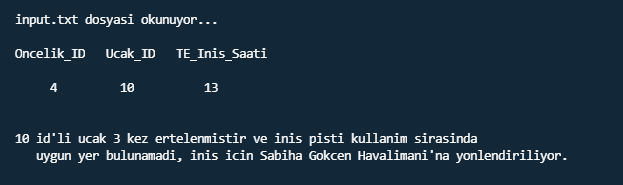
\includegraphics[scale=0.5]{img/go to sabiha message.png}
    \caption{uçak 3 kez ertelenir ve iniş için
   uygun yer bulunamayıp Sabiha Gokcen Havalimani'na yönlendirilir.}
    \label{Şekil:5}
\end{figure}
\begin{figure}[h]
    \centering
    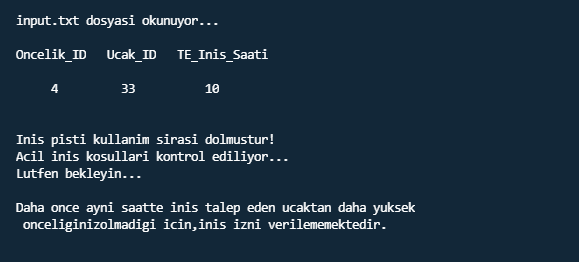
\includegraphics[scale=0.5]{img/message when landing list is full and incoming plane has lower priority.png}
    \caption{dizi doluysa ve gelen uçağın daha DÜŞÜK priority id'ye sahip olursa}
    \label{Şekil:6}
\end{figure}
\begin{figure}[h]
    \centering
    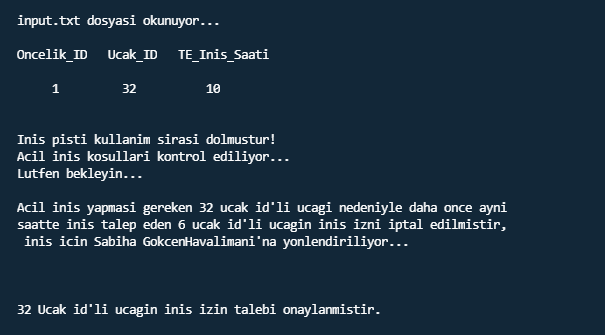
\includegraphics[scale=0.5]{img/message when landing list is full and incoming plane has higher priority(acil inis).png}
    \caption{dizi doluysa ve gelen uçağın daha YÜKSEK priority id'ye sahip olursa}
    \label{Şekil:7}
\end{figure}


%\subsection{\textbf{\Large Örtülü sonek ağacı oluşturma}}\label{AA}

\newpage
\section*{\textbf{\LARGE YALANCIKOD (PSEUDOCODES)}}
%\texttt{\textbf{Procedure} Min-Heapify(V, i)\\
\begin{figure}[h]
    \centering
    \includegraphics[scale=0.3]{img/1st pseudocode.jpeg}
\end{figure}
\begin{figure}[h]
    \centering
    \includegraphics[scale=0.3]{img/2nd pseudocode.jpeg}
\end{figure}
\begin{figure}[h]
    \centering
    \includegraphics[scale=0.4]{img/heap.jpeg}
\end{figure}
\\\\\\\\\\

\section*{\textbf{\LARGE Deneysel Sonuçlar}}

Havalimanına iniş yapacak uçaklar öncelikle kuleden iniş yapabilmek için izin talep eder. İniş izni talep eden her bir uçak için havalimanında yeterli kapasite olup olmadığı kontrol edilir. (inis\_pisti\_kullanim\_sirasi öncelikli kuyruğunda yeni uçak eklemek için boş alan var mı?). Kuleden iniş izni talep eden uçaklar için öncelikle, iniş talep edilen saatte pistin dolu mu boş mu olduğu kontrol edilir. Pist boş ise iniş yapılmak istenen saate izin verilir ve inis\_pisti\_kullanim\_sirasi’nda uygun yere eklenir. Aksi halde uçakların iniş sıralaması önceliğe göre belirlenir. Uçakların öncelik (oncelik\_id) sıralaması şu şekildedir (yüksekten düşüğe):

\begin{enumerate}
  \item Ambulans uçağı
  \item Savaş uçağı
  \item Yolcu uçağı 
  \item Kargo uçağı
\end{enumerate}

Tüm uçakların iniş ve kalkış süreleri eşittir ve hesaplamalara dâhil edilmeyecektir. Havalimanına iniş yapan her uçağın, kalkış için bekleme süresi 1 saattir. Uçakların kalkış saatine, ötelenmeden dolayı oluşan gecikme süreleri dâhil edilir. Kalkış saati bu bilgiler göz önünde bulundurularak hesaplanmıştır. Kuleden bir günde maksimum 24 uçak iniş için izin talep edebilir. Eğer bu kapasite dolmuşsa; o İniş için onay alan uçaklardan en az birinin önceliği (X uçağı olsun), iniş izni onayı bekleyen uçağın (Y uçağı olsun) önceliğinden düşükse; yüksek öncelikli yeni uçağa (Y) iniş onayı verilir. Daha önce onay almış ve önceliği düşük olan uçak (X) başka bir havalimanına yönlendirilecektir. O İniş izni daha önceden onaylanan uçağın (X) izni iptal edilmişse; “Acil iniş yapması gereken (Y) no’lu uçağı nedeniyle daha önce aynı saatte iniş talep eden (X) no’lu iniş izniniz iptal edilmiştir, iniş için Sabiha Gökçen Havalimanı’na yönlendiriliyor.” şeklinde ekranda yazdırılacaktır. İniş izni talep eden uçakların her biri satır satır input.txt’den okunur. Okunan her bir satır ekranda gösterilmektedir. Her yeni input satırı okunduğunda, kalkış yapacak olan uçakların bulunduğu output.txt dosyası güncellenir ve güncel kalkis\_pisti\_kullanim\_sirasi öncelikli kuyruğu ekranda gösterilir. 
output.txt dosyası uçakların kalkış saati bilgisine göre oluşturulmaktadır. Dosyanın içeriği şu şekildedir: 

\begin{itemize}
\item Her satırda oncelik\_id, ucak\_id, talep\_edilen\_inis\_saati, inis\_saati, gecikme\_suresi, kalkis\_saati olmak üzere toplamda 6 bilgi içermektedir. 
\item inis\_saati bilgisi; eğer uçak talep ettiği saatte iniş yapmışsa talep\_edilen\_inis\_saati ile aynıdır. Ancak talep edilen saatte önceliği yüksek başka bir uçak iniş yapacaksa belirlenen yeni iniş saati, kalkış saatinin hesaplanmasında kullanılmaktadır. 
\item Bilgiler input.txt’de olduğu gibi boşluk ile ayrılmaktadır.
\end{itemize}

Projede kullanılmış olan veri yapıları aşağıdaki gibidir: 
\begin{itemize}
\item PlaneL (inis\_pisti\_kullanim\_sirasi): Havalimanına iniş yapacak uçakların iniş pistini kullanım sırasını içeren öncelikli kuyruktur. Uçak öncelik ve iniş saati bilgisi dikkate alınarak hazırlanmıştır.
\item PlaneT (kalkis\_pisti\_kullanim\_sirasi): Havalimanından kalkış yapacak uçakların kalkış pistini kullanım sırasını içeren öncelikli kuyruktur. Uçak öncelik ve kalkış saati bilgisine göre hazırlanmıştır.
\end{itemize}

\begin{figure}[h]
    \centering
    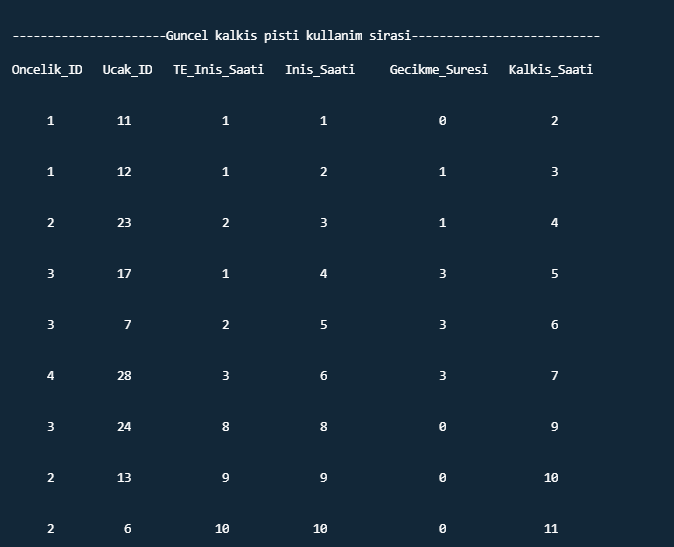
\includegraphics[scale=0.5]{img/the last guncel kalkis pisti kullanim sirasi p1.png}
    \caption{ Güncel kalkış pisti kullanım süresi }
\end{figure}

\begin{figure}[h]
    \centering
    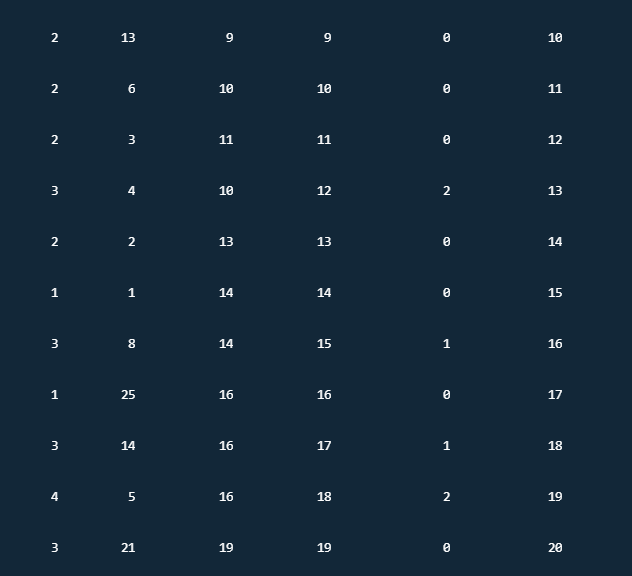
\includegraphics[scale=0.5]{img/the last guncel kalkis pisti kullanim sirasi p2.png}
    \caption{}
\end{figure}

\begin{figure}[h]
    \centering
    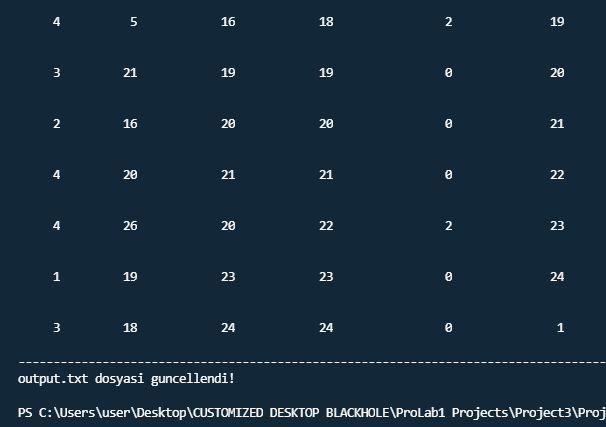
\includegraphics[scale=0.5]{img/the last guncel kalkis pisti kullanim sirasi p3.png}
    \caption{}
\end{figure}

\newpage

\section*{\LARGE Kaynakça}
\begin{thebibliography}{00}
\normalsize
\bibitem{b1} https://medium.com/@tolgahan.cepel/do\%C4\%9Frusal-veri-yap\%C4\%B1lar\%C4\%B1-4-kuyruk-queue-dcbd07e8ba77

\bibitem{b2} https://www.geeksforgeeks.org/priority-queue-set-1-introduction/
\bibitem{b3} https://www.programiz.com/dsa/priority-queue

\bibitem{b4} https://docs.oracle.com/javase/7/docs/api/java/util/PriorityQueue.html
\bibitem{b5} https://www.programiz.com/dsa/heap-data-structure

\bibitem{b6} https://www.geeksforgeeks.org/binary-heap/


\bibitem{7} https://www.sanfoundry.com/c-program-implement-heap/
\bibitem{8} https://www.youtube.com/watch?v=HqPJF2L5h9U&t=1335s
\bibitem{9} https://www.youtube.com/watch?v=wptevk0bshY
\bibitem{10} https://www.youtube.com/watch?v=\_U1AJZQxYTU
\bibitem{11} https://www.codesansar.com/c-programming/recursive-function.htm
\bibitem{12} https://www.tutorialspoint.com/cprogramming/c\_recursion.htm
\bibitem{13} https://www.programiz.com/c-programming/c-recursion
\bibitem{14} https://www.youtube.com/watch?v=kepBmgvWNDw

\bibitem{15} Book Algorithms on Strings, Trees and Sequences: Computer Science and Computational Biology by Dan Gusfield
\bibitem{16} https://www.youtube.com/watch?v=ngCos392W4w
\bibitem{17} https://www.youtube.com/watch?v=ggk7HbcnLG8
\bibitem{18} https://www.youtube.com/watch?v=QWDCKPEWSWo&t=425s
\bibitem{19} https://www.youtube.com/watch?v=cv7CY8UmFL0
\bibitem{20} https://www.geeksforgeeks.org/readwrite-structure-file-c/
\bibitem{21} https://cboard.cprogramming.com/c-programming/77351-writing-array-struct-file.html

\bibitem{22} https://courses.cs.washington.edu/courses/cse373/17wi/lectures/priority-queues.pdf
\bibitem{23} http://www.cs.cornell.edu/courses/cs2110/2015fa/L17-PriorityQueuesAndHeaps/cs2110PqueuesHeaps.pdf
\bibitem{24} https://www.geeksforgeeks.org/priority-queue-using-binary-heap/
\bibitem{25} https://runestone.academy/runestone/books/published/pythonds/Trees/BinaryHeapImplementation.html
\bibitem{26} https://www.hackerearth.com/practice/notes/heaps-and-priority-queues/
\bibitem{27} https://algs4.cs.princeton.edu/24pq/
\bibitem{28} https://cgi.csc.liv.ac.uk/~leszek/COMP202/week4/week4.pdf
\bibitem{2} https://www.overleaf.com/

\end{thebibliography}


\end{document}
